\section{Introduction}
\label{sec:intro}

Distribution shifts---where the training distribution differs from the test distribution---can significantly degrade the accuracy of machine learning (ML) systems deployed in the wild.
In this work, we consider two types of distribution shifts that are ubiquitous in real-world settings: domain generalization and subpopulation shift (\reffig{problems}).
In \emph{domain generalization}, the training and test distributions comprise data from related but distinct domains. This problem arises naturally in many applications, as it is often infeasible to collect a training set that spans all domains of interest. For example, in medical applications, it is common to seek to train a model on patients from a few hospitals, and then deploy it more broadly to hospitals outside the training set \citep{zech2018radio}; and in wildlife monitoring, we might seek to train an animal recognition model on images from one set of camera traps and then deploy it to new camera traps \citep{beery2018recognition}.
In \emph{subpopulation shift}, we consider test distributions that are subpopulations of the training distribution, with the goal of doing well even on the worst-case subpopulation.
For example, it is well-documented that standard models often perform poorly on under-represented demographics \citep{buolamwini2018gender,koenecke2020racial},
and so we might seek models that can perform well on all demographic subpopulations.

\begin{figure}[!b]
  \centering
  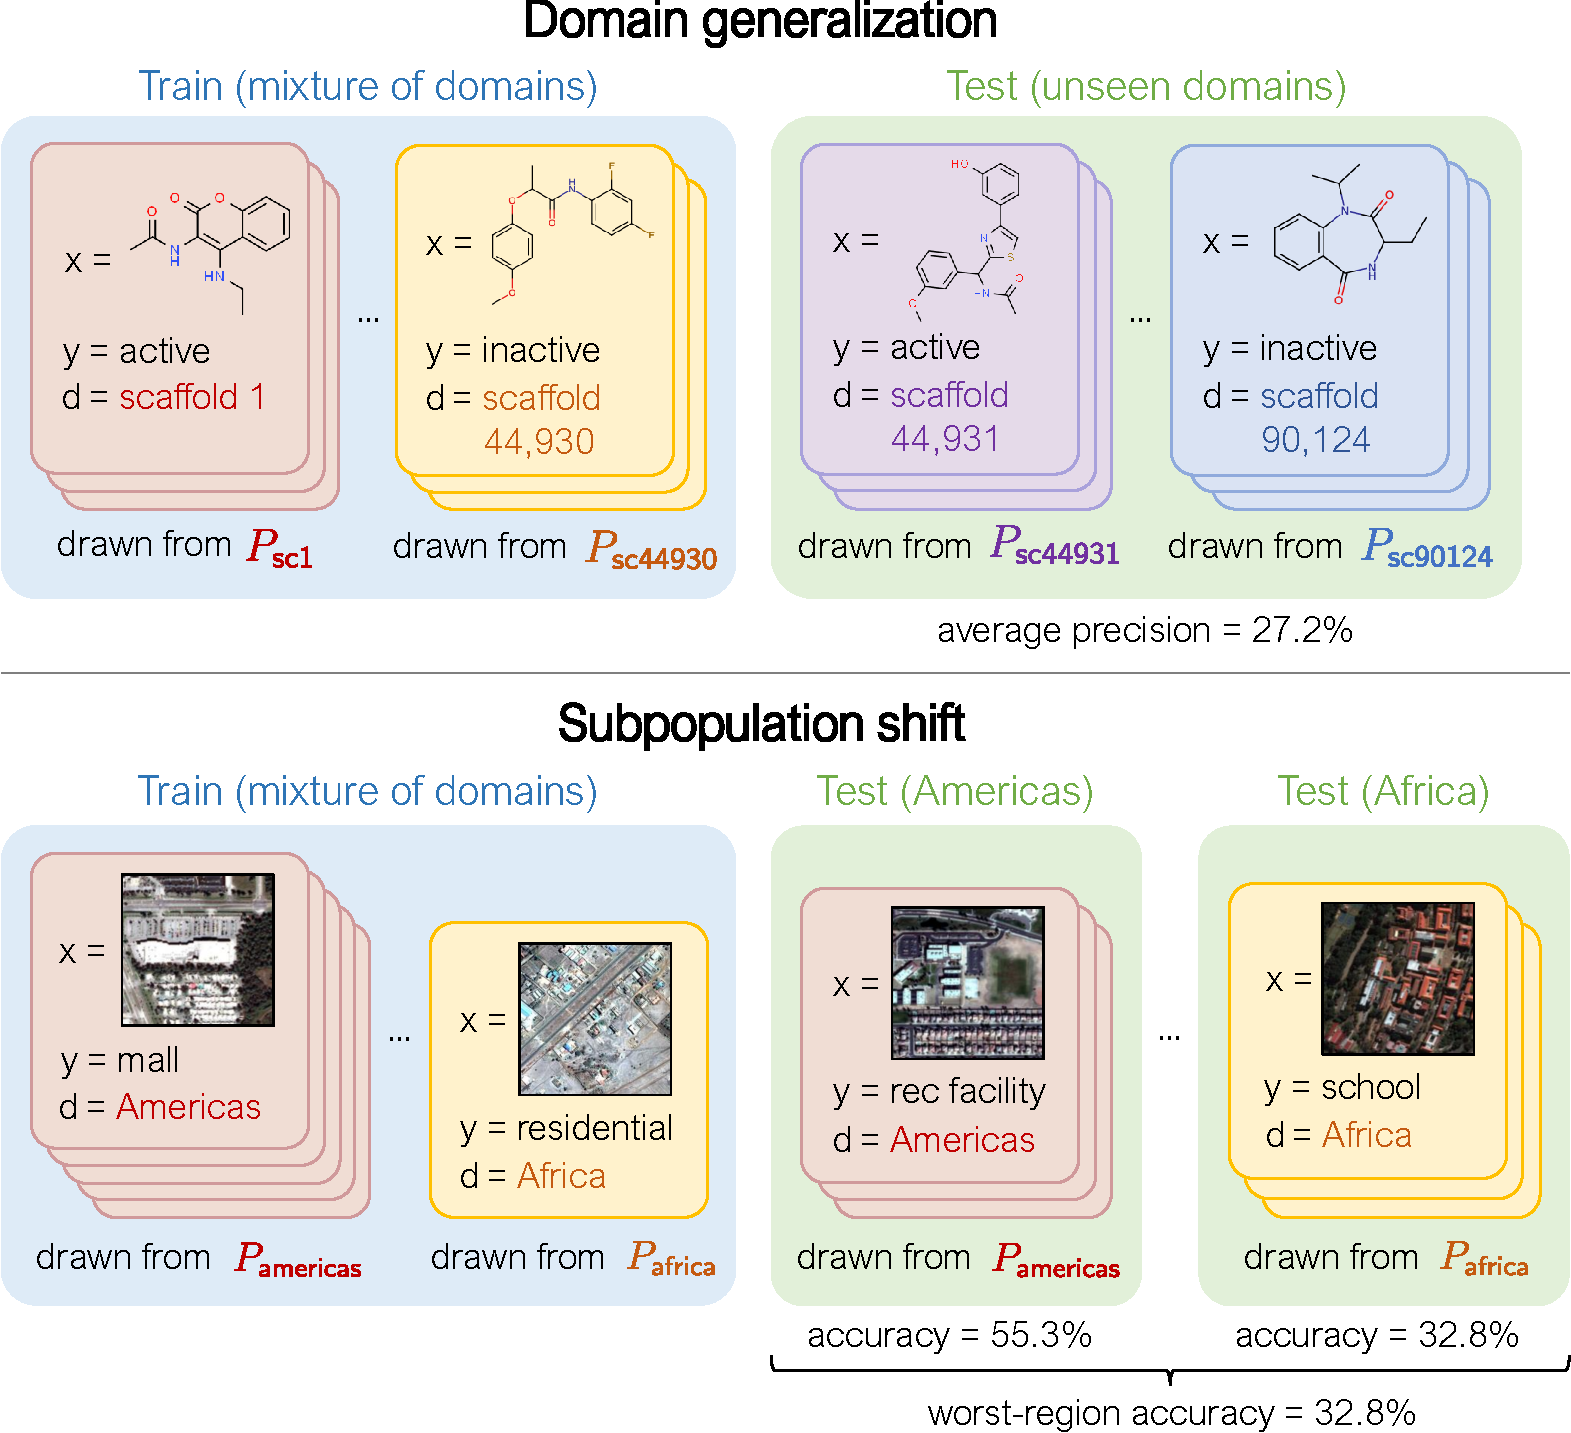
\includegraphics[width=0.75\linewidth]{figures/problem_overview.pdf}
  \caption{
    In each \Wilds dataset, each data point $(x,y,\dom)$ is associated with a domain $\dom$.
    Each domain corresponds to a distribution $\Pdom$ over data points which are similar in some way, e.g., molecules with the same scaffold, or satellite images from the same region.
    We study two types of distribution shifts.
    \textbf{Top:} In \emph{domain generalization}, we train and test on disjoint sets of domains. The goal is to generalize to domains unseen during training, e.g., molecules with a new scaffold in \Mol \citep{hu2020open}.
    \textbf{Bottom:} In \emph{subpopulation shift}, the training and test domains overlap, but their relative proportions differ. We typically assess models by their worst performance over test domains, each of which correspond to a subpopulation of interest, e.g., different geographical regions in \FMoW \citep{christie2018fmow}.
    }
  \label{fig:problems}
\end{figure}

\begin{figure*}[!t]
  \centering
  \makebox[\textwidth][c]{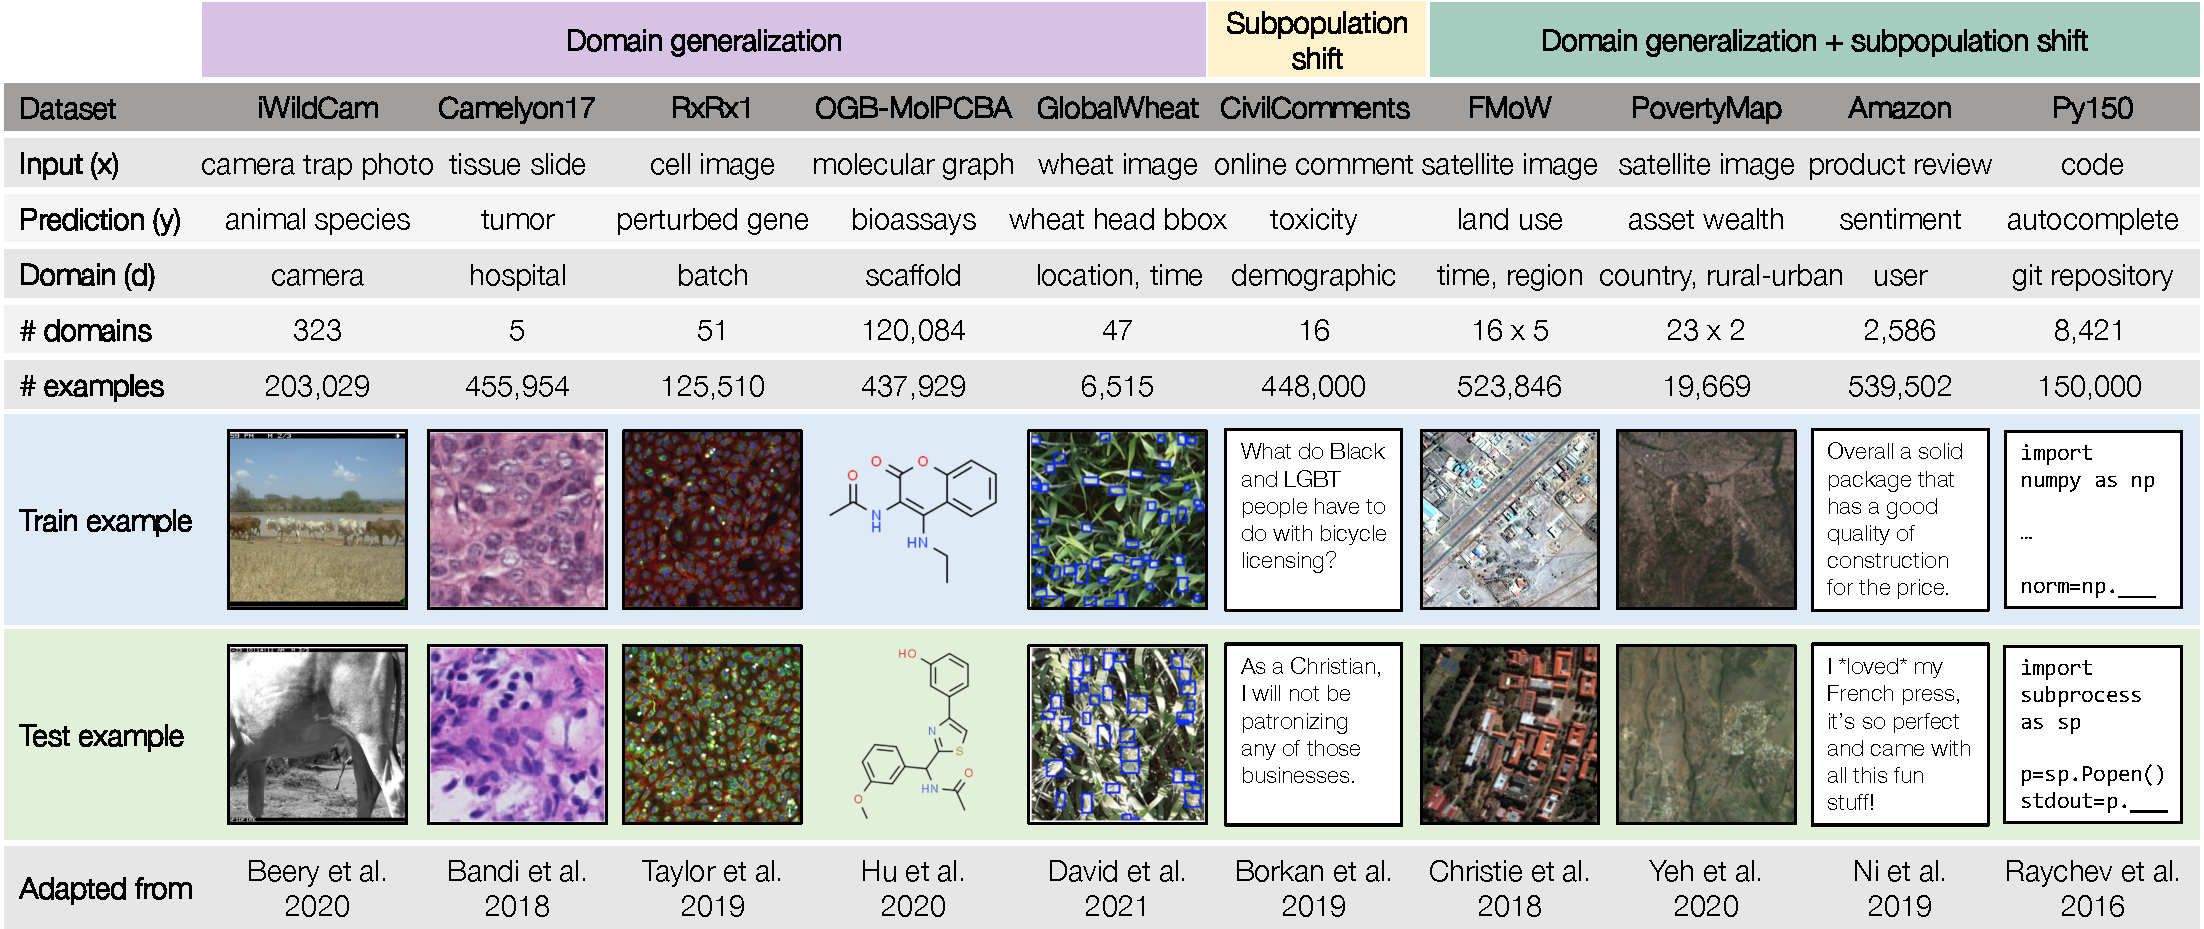
\includegraphics[width=1.1\textwidth]{figures/datasets_summary.pdf}}
  \caption{
    The \Wilds benchmark contains 10 datasets across a diverse set of application areas, data modalities, and dataset sizes. Each dataset comprises data from different domains, and the benchmark is set up to evaluate models on distribution shifts across these domains.
    }
  \label{fig:datasets}
\end{figure*}

Despite their ubiquity in real-world deployments, these types of distribution shifts are under-represented in the datasets widely used in the ML community today \citep{geirhos2020shortcut}.
Most of these datasets were designed for the standard i.i.d. setting, with training and test sets from the same distribution,
and prior work on retrofitting them with distribution shifts has focused on shifts that are cleanly characterized but not always likely to arise in real-world deployments.
For instance, many recent papers have studied datasets with shifts induced by synthetic transformations, such as changing the color of MNIST digits \citep{arjovsky2019invariant}, or by disparate data splits, such as generalizing from cartoons to photos \citep{li2017deeper}.
Datasets like these are important testbeds for systematic studies, but they do not generally reflect the kinds of shifts that are likely to arise in the wild.
To develop and evaluate methods for real-world shifts, we need to complement these datasets with benchmarks that capture shifts in the wild, as model robustness need not transfer across shifts: e.g., models can be robust to image corruptions but not to shifts across datasets \citep{taori2020measuring, djolonga2020robustness}, and a method that improves robustness on a standard vision dataset can even consistently harm robustness on real-world satellite imagery datasets \citep{xie2020innout}.

In this paper, we present \Wilds, a curated benchmark of 10 datasets with evaluation metrics and train/test splits representing a broad array of distribution shifts that ML models face in the wild (\reffig{datasets}). With \Wilds, we seek to complement existing benchmarks by focusing on datasets with realistic shifts across a diverse set of data modalities and applications:
animal species categorization \citep{beery2020iwildcam},
tumor identification \citep{bandi2018detection},
bioassay prediction \citep{wu2018moleculenet,hu2020open},
genetic perturbation classification \citep{taylor2019rxrx1},
wheat head detection \citep{david2020global},
text toxicity classification \citep{borkan2019nuanced},
land use classification \citep{christie2018fmow},
poverty mapping \citep{yeh2020poverty},
sentiment analysis \citep{ni2019justifying},
and code completion \citep{raychev2016probabilistic,CodeXGLUE}.
These datasets reflect natural distribution shifts arising from different cameras, hospitals, molecular scaffolds, experiments, demographics, countries, time periods, users, and codebases.

\Wilds builds on extensive data-collection efforts by domain experts, who are often forced to grapple with distribution shifts to make progress in their applications.
To design \Wilds, we worked with them to identify, select, and adapt datasets that fulfilled the following criteria:
\begin{enumerate}
  \item \textbf{Distribution shifts with performance drops.} The train/test splits reflect shifts that substantially degrade model performance,
  i.e., with a large gap between in-distribution and out-of-distribution performance.
  \item \textbf{Real-world relevance.} The training/test splits and evaluation metrics are motivated by real-world scenarios and chosen in conjunction with domain experts. In \refapp{app_realism}, we further discuss the framework we use to assess the realism of a dataset.
  \item \textbf{Potential leverage.} Distribution shift benchmarks must be non-trivial but also possible to solve, as models cannot be expected to generalize to arbitrary distribution shifts. We constructed each \Wilds dataset to have training data from multiple domains, with domain annotations and other metadata available at training time. We hope that these can be used to learn robust models: e.g., for domain generalization, one could use these annotations to learn models that are invariant to domain-specific features \citep{sun2016deep,ganin2016domain}, while for subpopulation shift, one could learn models that perform uniformly well across each subpopulation \citep{hu2018does,sagawa2020group}.
\end{enumerate}
We chose the \Wilds datasets to collectively encompass a diverse set of tasks, data modalities, dataset sizes, and numbers of domains, so as to enable evaluation across a broad range of real-world distribution shifts.
In \refsec{other_datasets}, we further survey the distribution shifts that occur in other application areas---algorithmic fairness and policing, medicine and healthcare, genomics, natural language and speech processing, education, and robotics---and discuss examples of datasets from these areas that we considered but did not include in \Wilds, as their distribution shifts did not cause an appreciable performance drop.

To make the \Wilds datasets more accessible, we have substantially modified most of them to clarify the distribution shift, standardize the data splits, and preprocess the data for use in standard ML frameworks.
In \refsec{library}, we introduce our accompanying open-source Python package that fully automates data loading and evaluation. The package also includes default models appropriate for each dataset, allowing all of the baseline results reported in this paper to be easily replicated.
To track the state-of-the-art in training algorithms and model architectures that are robust to these distribution shifts, we are also hosting a public leaderboard; we discuss guidelines for developers in \refsec{guidelines}.
Code, leaderboards, and updates are available at \url{https://wilds.stanford.edu}.

Datasets are significant catalysts for ML research.
Likewise, benchmarks that curate and standardize datasets---e.g., the GLUE and SuperGLUE benchmarks for language understanding \citep{wang2019superglue,wang2019glue} and the Open Graph Benchmark for graph ML \citep{hu2020open}---can accelerate research by focusing community attention, easing development on multiple datasets, and enabling systematic comparisons between approaches.
In this spirit, we hope that \Wilds will facilitate the development of ML methods and models that are robust to real-world distribution shifts and can therefore be deployed reliably in the wild.
